\chapter{Results}

We outline the results of the method first by validating that each step of
the method had plausible outputs, and then by reporting the estimated
parameters based on the observed data.

\section{Validation}

\begin{table}[htbp]
    \caption{
        Final Gaussian process hyperparameters
    }
    \label{tab:trained_hps}
    \centering
    \begin{tabular}{c|c}
        Hyperparameter    & Final value \\
        $\sigma_o^2$      & $0.07$      \\
        $\sigma_k^2$      & $0.707$     \\
        $\ell_\alpha$     & $0.324$     \\
        $\ell_\beta$      & $0.715$     \\
        $\ell_{\gamma_L}$ & $0.010$     \\
        $\ell_\lambda$    & $0.006$     \\
        $\ell_f$          & $0.016$     \\
        $\ell_r$          & $0.016$     \\
        $m_\GP$           & $0.879$
    \end{tabular}
\end{table}

\begin{figure}[htbp]
    \centering
    \begin{minipage}[b]{0.33\textwidth}
        \centering
        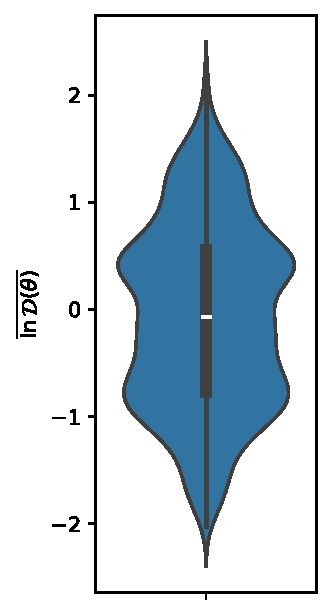
\includegraphics[width=\textwidth]{discreps_violin.pdf}
        \caption{$\smtheta$ violin plot}
        \label{fig:violin}
    \end{minipage}
    \begin{minipage}[b]{0.66\textwidth}
        \centering
        \begin{minipage}[b]{\textwidth}
            \centering
            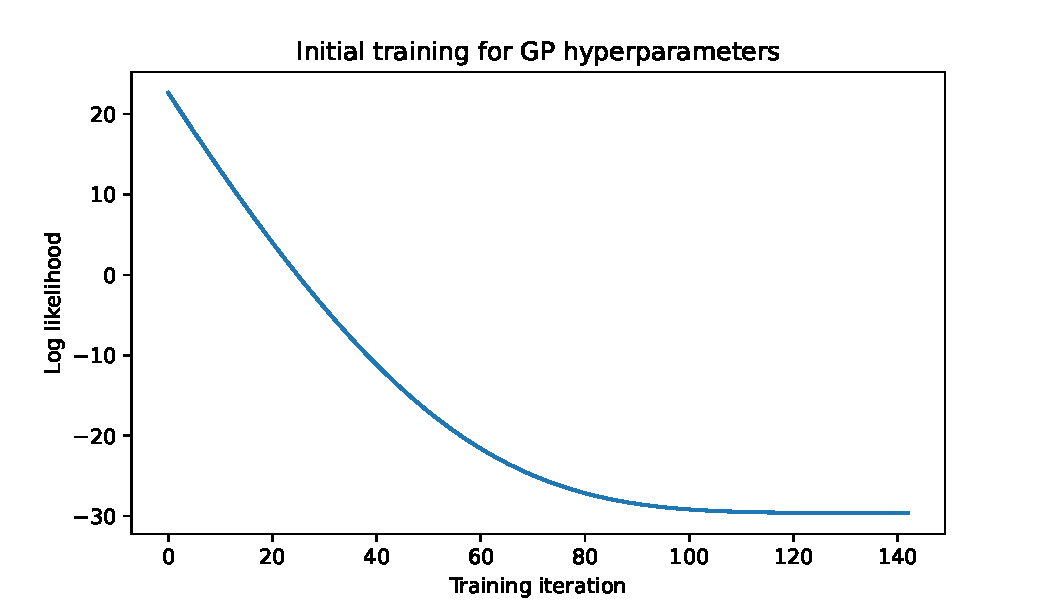
\includegraphics[width=\textwidth]{hyperparam_loss_log_discrep.pdf}
            \caption{Hyperparameter training}
            \label{fig:hyper_train}
        \end{minipage}
        \begin{minipage}[b]{\textwidth}
            \centering
            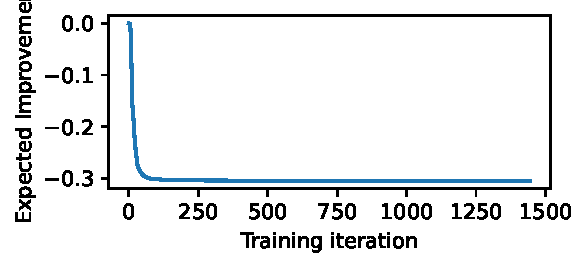
\includegraphics[width=\textwidth]{initial_EI_loss_training.pdf}
            \caption{Finding $\argmin_{\btheta}\A_\EI(\btheta)$}
            \label{fig:subEI}
        \end{minipage}
    \end{minipage}
    % \caption{
    %     Validation of the results from training the Gaussian process. The
    %     \textcolor{red}{something about the discrepancy values being spread}.
    %     }
    % \label{fig:validation}
\end{figure}

The final hyperparameters, are reported in Table \ref{tab:trained_hps}.
To ensure that our expected improvement and hyperparameter optimisation 
functions converged, we plotted the initial trainings in 
Figures \ref{fig:hyper_train} and \ref{fig:subEI}. The plots have a 
smooth curve, demonstrating that both algorithms converged at a good
rate.

The violin plot of discrepancy function in Figure \ref{fig:violin}
is well dispersed suggesting a good
amount of exploration of the parameter space has been done. A large number
of samples were in areas of low mean log discrepancy, and so 
this suggests a good exploration exploitation trade-off.

\begin{figure}[htbp]
    \centering
    \begin{subfigure}[b]{0.5\textwidth}
        \centering
        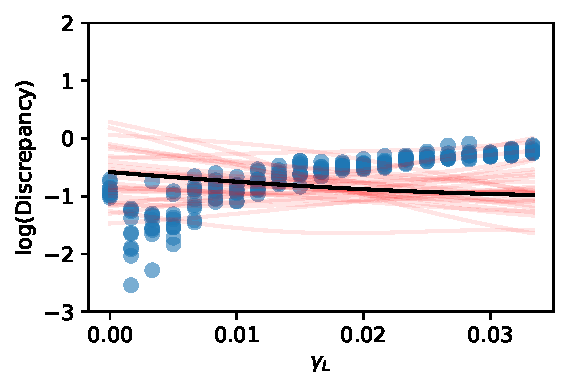
\includegraphics[width=\textwidth]{
            ../champagne_GP_images/initial_gamma_L_slice_log_discrep.pdf
        }
    \end{subfigure}%
    \hfill%
    \begin{subfigure}[b]{0.5\textwidth}
        \centering
        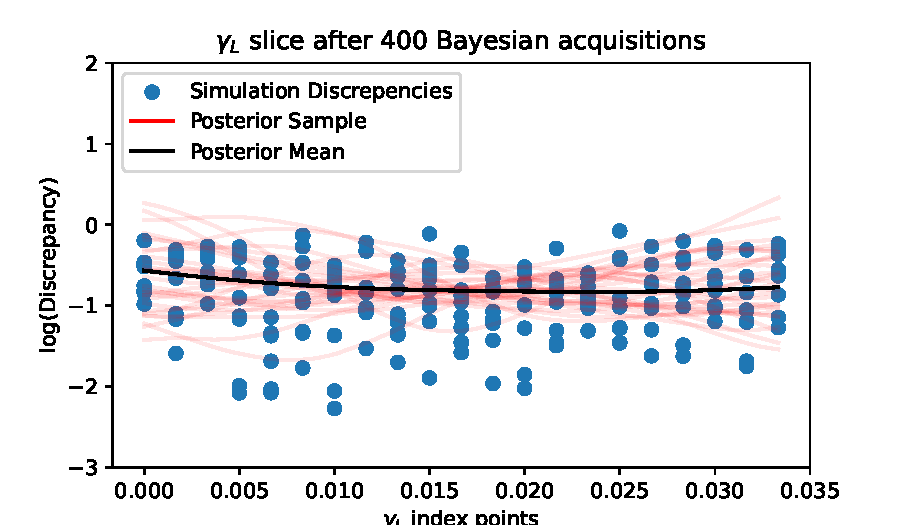
\includegraphics[width=\textwidth]{
            ../champagne_GP_images/gamma_L_slice_400_bolfi_updates_log_discrep.pdf
        }
    \end{subfigure}
    \hfill%
    \begin{subfigure}[b]{0.5\textwidth}
        \centering
        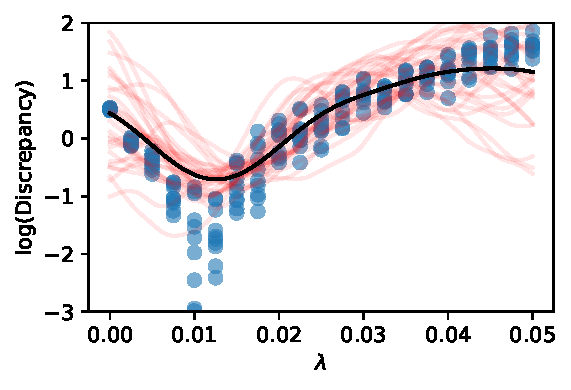
\includegraphics[width=\textwidth]{
            ../champagne_GP_images/initial_lambda_slice_log_discrep.pdf
        }
    \end{subfigure}%
    \hfill%
    \begin{subfigure}[b]{0.5\textwidth}
        \centering
        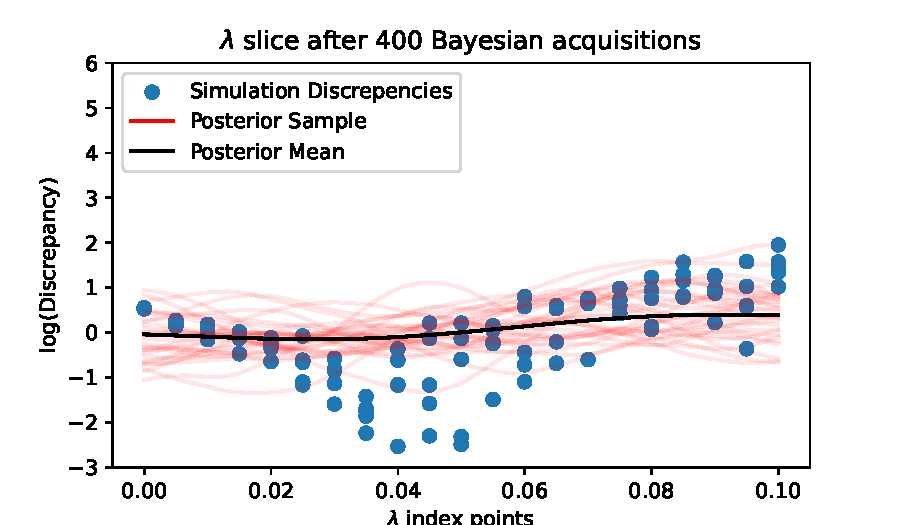
\includegraphics[width=\textwidth]{
            ../champagne_GP_images/lambda_slice_400_bolfi_updates_log_discrep.pdf
        }
    \end{subfigure}
    \begin{subfigure}[b]{0.5\textwidth}
        \centering
        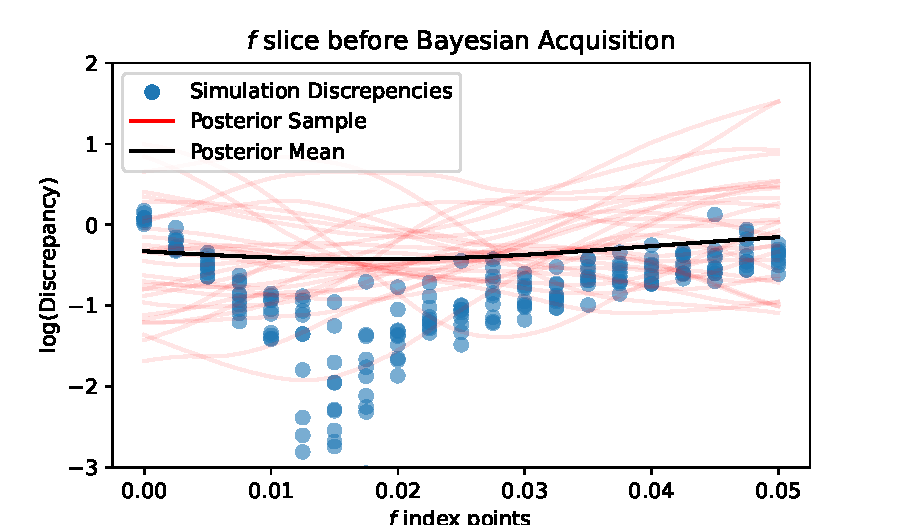
\includegraphics[width=\textwidth]{
            ../champagne_GP_images/initial_f_slice_log_discrep.pdf
        }
    \end{subfigure}%
    \hfill%
    \begin{subfigure}[b]{0.5\textwidth}
        \centering
        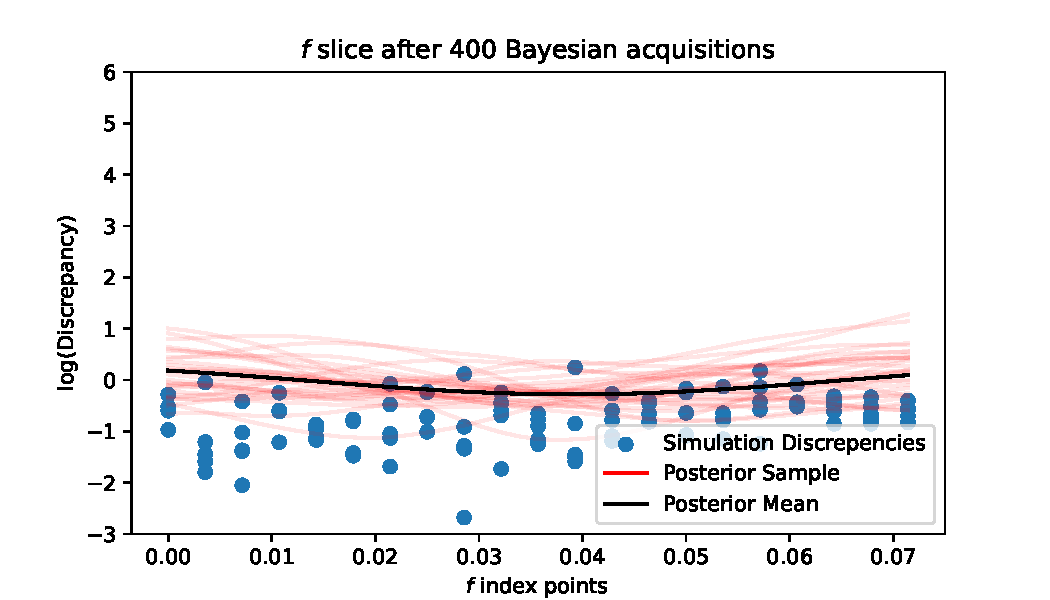
\includegraphics[width=\textwidth]{
            ../champagne_GP_images/f_slice_400_bolfi_updates_log_discrep.pdf
        }
    \end{subfigure}
    \hfill%
    \begin{subfigure}[b]{0.5\textwidth}
        \centering
        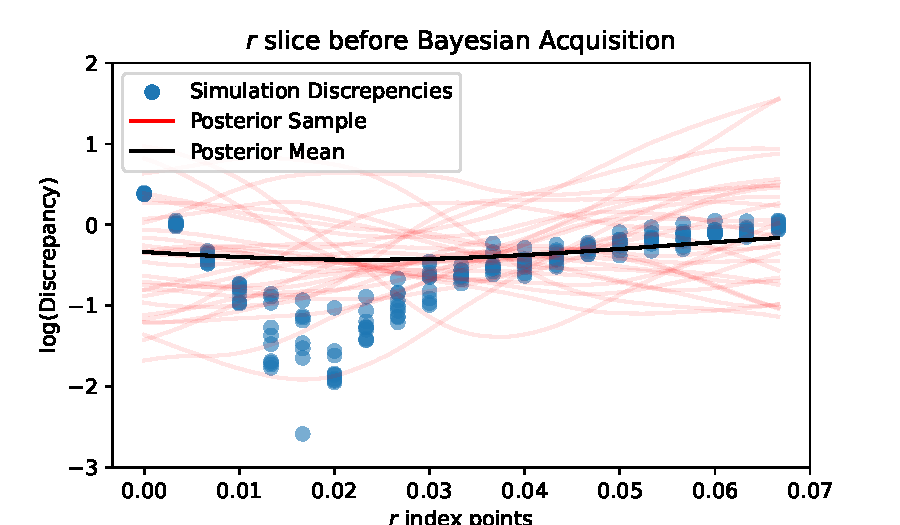
\includegraphics[width=\textwidth]{
            ../champagne_GP_images/initial_r_slice_log_discrep.pdf
        }
    \end{subfigure}%
    \hfill%
    \begin{subfigure}[b]{0.5\textwidth}
        \centering
        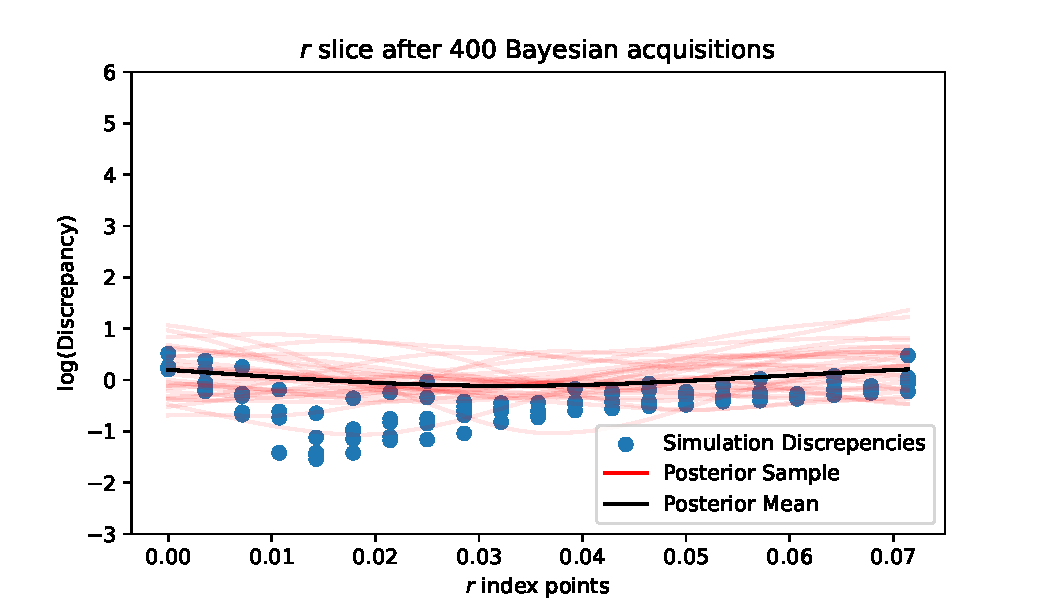
\includegraphics[width=\textwidth]{
            ../champagne_GP_images/r_slice_400_bolfi_updates_log_discrep.pdf
        }
    \end{subfigure}
    \caption{
        The left column of figures is the Gaussian process after initialisation
        $d_\GP^{(0)}(\btheta).$ The black line is $\E(d_\GP^{(0)}(\btheta)),$
        and the red lines are multiple realisations of
        $d_\GP^{(0)}(\btheta).$ The right column of figures is after 400
        sampling iterations, with the black line being
        $\E(d_\GP^{(400)}(\btheta)).$
        The blue dots are realisations of $\ln\mathcal{D}(\bm{\theta}).$
        $d_\GP$ has not been trained on these realisations.
        The parameters are varied
        univariately, with all other parameters fixed at the true parameters.
    }
    \label{fig:improving_GP}
\end{figure}

\begin{figure}[htbp]
    \centering
    \begin{subfigure}[b]{0.5\textwidth}
        \centering
        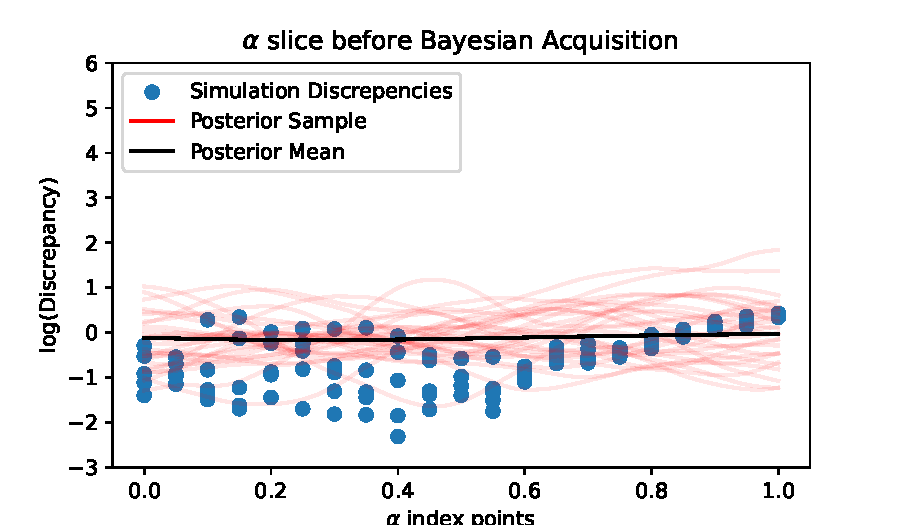
\includegraphics[width=\textwidth]{
            ../champagne_GP_images/initial_alpha_slice_log_discrep.pdf
        }
    \end{subfigure}%
    \hfill%
    \begin{subfigure}[b]{0.5\textwidth}
        \centering
        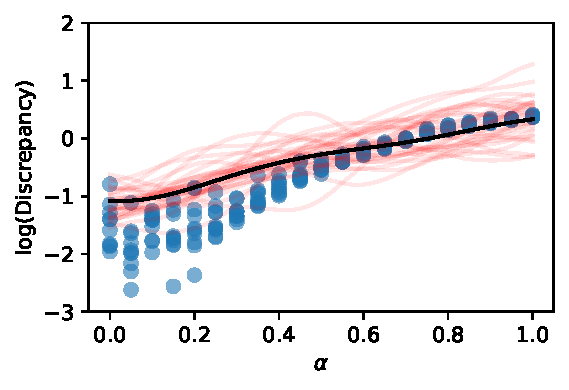
\includegraphics[width=\textwidth]{
            ../champagne_GP_images/alpha_slice_400_bolfi_updates_log_discrep.pdf
        }
    \end{subfigure}
    \hfill%
    \begin{subfigure}[b]{0.5\textwidth}
        \centering
        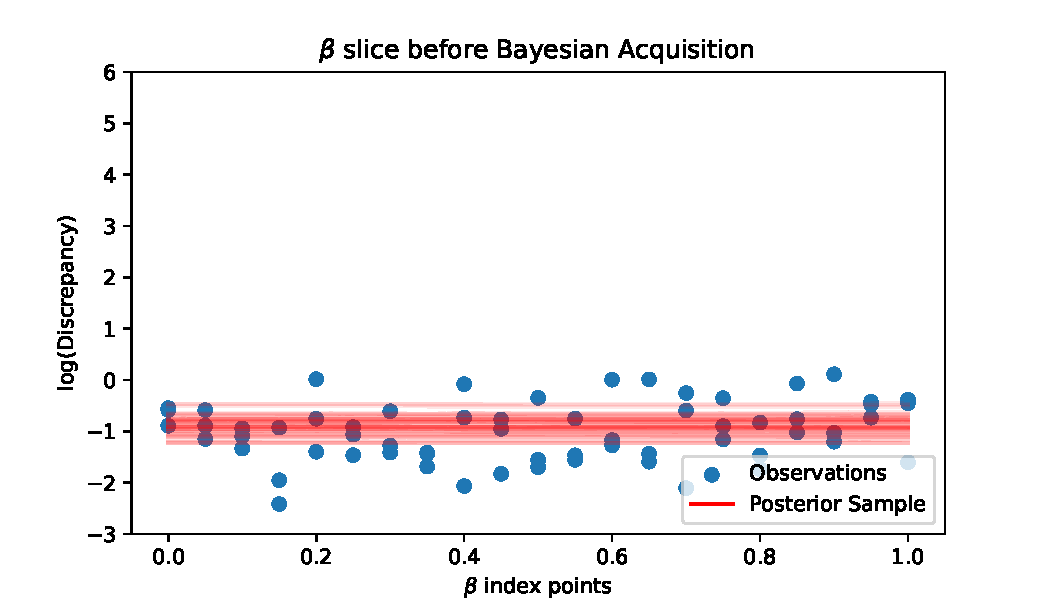
\includegraphics[width=\textwidth]{
            ../champagne_GP_images/initial_beta_slice_log_discrep.pdf
        }
    \end{subfigure}%
    \hfill%
    \begin{subfigure}[b]{0.5\textwidth}
        \centering
        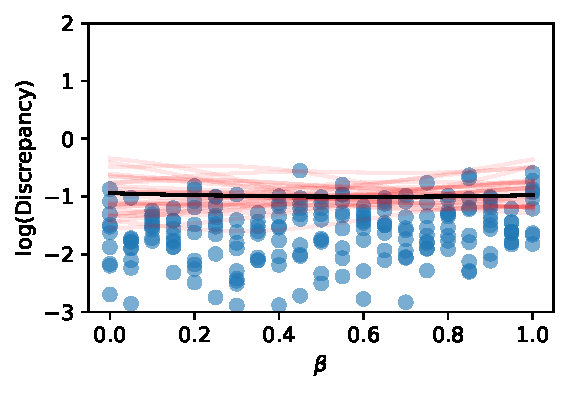
\includegraphics[width=\textwidth]{
            ../champagne_GP_images/beta_slice_400_bolfi_updates_log_discrep.pdf
        }
    \end{subfigure}
    \caption{
        Gaussian process approximations of the treatment parameters, as with
        Figure \ref{fig:improving_GP}
    }
    \label{fig:treatment_GP_fig}
\end{figure}

Figure \ref{fig:improving_GP} suggests that after 400 iterations
$d_\GP(\btheta)$ fits to $\E(\ln\D(\btheta))$ well.
The $\lambda$ slice has the sharpest minimum, whereas $\beta$
does not appear to have much impact on the discrepancy.
As the number of iterations increased, the Gaussian process visibly
improved at fitting to the mean. Interim iterations of $d^{(t)}_\GP(\btheta)$
can be seen in the appendix.

\section{Parameter estimation}

\begin{figure}[htbp]
    \centering
    \begin{subfigure}[b]{0.5\textwidth}
        \centering
        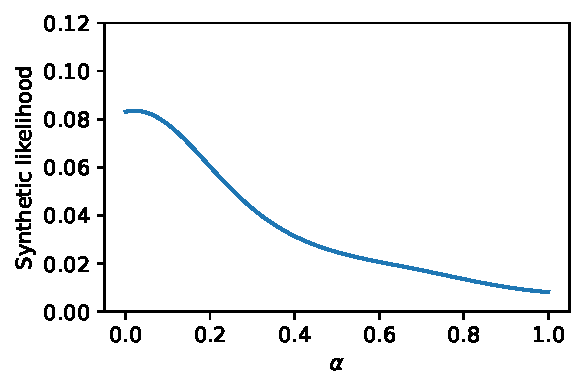
\includegraphics[width=\textwidth]{alpha_slice_synth_likelihood.pdf}
    \end{subfigure}%
    \hfill%
    \begin{subfigure}[b]{0.5\textwidth}
        \centering
        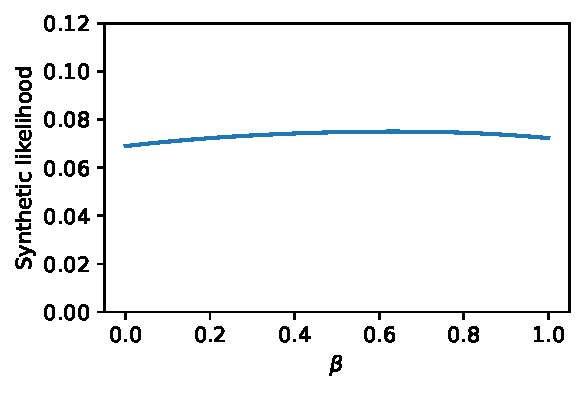
\includegraphics[width=\textwidth]{beta_slice_synth_likelihood.pdf}
    \end{subfigure}
    \begin{subfigure}[b]{0.5\textwidth}
        \centering
        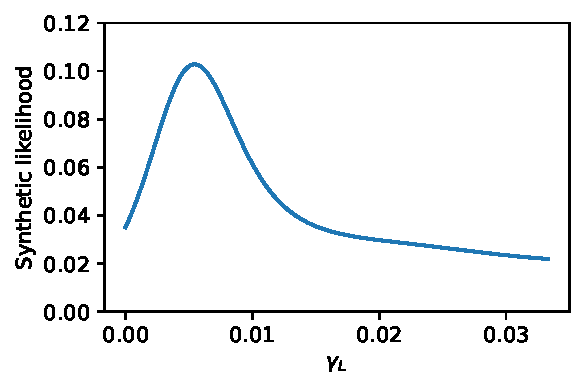
\includegraphics[width=\textwidth]{gamma_L_slice_synth_likelihood.pdf}
    \end{subfigure}%
    \hfill%
    \begin{subfigure}[b]{0.5\textwidth}
        \centering
        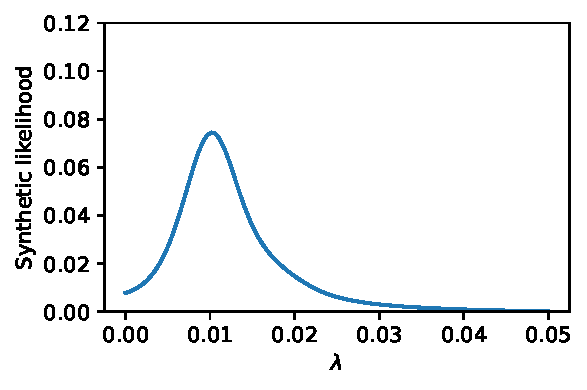
\includegraphics[width=\textwidth]{lambda_slice_synth_likelihood.pdf}
    \end{subfigure}
    \begin{subfigure}[b]{0.5\textwidth}
        \centering
        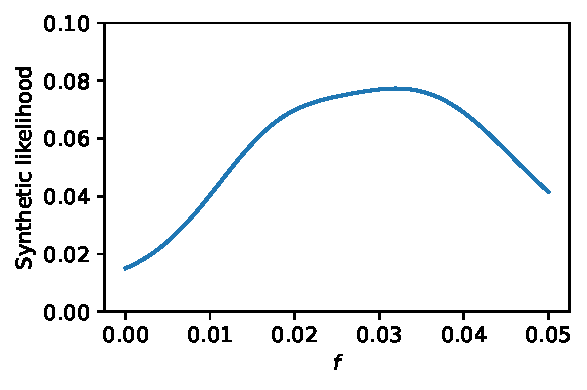
\includegraphics[width=\textwidth]{f_slice_synth_likelihood.pdf}
    \end{subfigure}%
    \hfill%
    \begin{subfigure}[b]{0.5\textwidth}
        \centering
        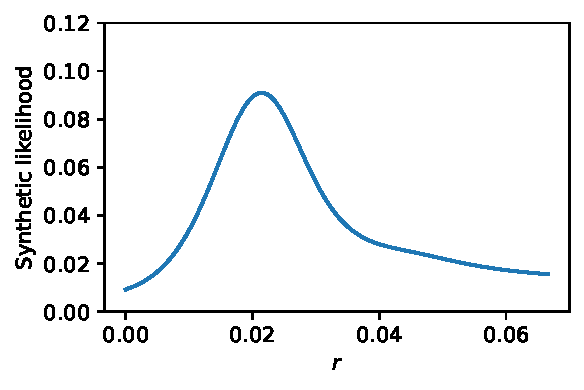
\includegraphics[width=\textwidth]{r_slice_synth_likelihood.pdf}
    \end{subfigure}%
    \caption{
        Final univariate synthetic likelihoods $\hat{L}(\bm{\theta})$ after
        400 sampling iterations. All values not shown were fixed at the true
        parameters.
    }
    \label{fig:final_synth_lik}
\end{figure}

\begin{table}[htbp]
    \caption{
        Estimates of our model parameters.
        The maximum likelihood estimate (MLE) of the true parameters using
        $\hat{L}.$ The maximum slice estimate was the one-dimensional
        maximum likelihood estimate where all other parameters are held
        constant at the true value.
    }
    \label{tab:param_est}
    \centering
    \begin{tabular}{c | c | c | c}
        Parameter  & True     & MLE     & ML Slice Estimate \\
        \hline
        $\alpha$   & $0.124$  & $0.153$ & $0.02$            \\
        $\beta $   & $0.429$  & $0.555$ & $0.63$            \\
        $\gamma_L$ & $0.0026$ & $0.006$ & $0.005$           \\
        $\lambda$  & $0.01$   & $0.01$  & $0.01$            \\
        $f$        & $0.014$  & $0.024$ & $0.017$           \\
        $r$        & $0.017$  & $0.023$ & $0.022$           \\
    \end{tabular}
\end{table}

For parameter estimation, we typically look at likelihood instead of 
discrepancy. This is done by inverting 
that distribution function (see Equation \ref{eq:fin_lik}). 
In Table \ref{tab:param_est} we present the global maximum 
likelihood estimate found by finding the maximum synthetic likelihood 
$\argmax_{\btheta}\hat{L}(\btheta).$

In Figure \ref{fig:final_synth_lik} we show our final likelihood function 
estimate from the trained Gaussian process.
For simplicity we only present the likelihood across parameter slices, where 
the parameter of 
interest is allowed to vary, while all other parameters are held constant at
their true values. The maximum likelihood values for each parameter slice
is also presented in Table \ref{tab:param_est}, but do not vary much from the
maximum likelihood estimates, and the true values. For this reason, 
we can be confident that our synthetic likelihood is a good approximation of
the true likelihood, despite the true likelihood being infeasible to compare
to. Certain parameters such as $\lambda,$ $r,$ and $\gamma_L$ have sharper 
likelihood peaks than parameters such as $\alpha$ and $\beta,$ suggesting the
data we used may lend itself to estimating parameters such as $\lambda$ over
the treatment parameters, although all likelihood slices calculated were
unimodal.

\chapter{Discussion}

To our knowledge, the use of the synthetic likelihood as described above
has not been used to calibrate a malaria model before.
\Citeauthor{champagne_using_2022} calibrate the model we use
by finding the ODE equilibrium, and fitting a single parameter $\lambda$ to
incidence data. 
Note that this comes with limitations. For example, this relies on data being
observed when the disease is roughly at equilibria in the population.
This is not desirable for modelling outbreaks or seasonality effects.
\Citeauthor{champagne_using_2022}'s approach parameter calibration 
does not work in these scenarios.

In comparison, not only were we able to effectively
recover the true $\lambda$ from a synthetic run, we were able to recover
all model parameters simultaneously.

This methodology is very robust to both frequentist and Bayesian inference.
Under a Bayesian framework,
since we can evaluate the synthetic likelihood for any $\btheta,$
we can use a Metropolis Hasting sampler, to obtain samples from a distribution
approximately equal to the posterior distribution $\Pr(\btheta | \by^\obs).$
Alternatively, standard frequentist inference can also be used on our
synthetic likelihood $\hat{L}.$ For example, numerically approximating the
observed Fisher information matrix
$$
    F(\hat{\theta})
    = -\frac{\partial \ln\hat{L}}{\partial \btheta\partial \btheta^T}(\hat{\btheta})
$$
allows us to do hypothesis testing and construct confidence intervals,
since asymptotically $\hat{\btheta} \sim N(\btheta, F^{-1}(\hat{\btheta}))$
(see \cite{fahrmeir_multivariate_2013}).

Although the likelihood free procedure we outlined for this model closely
resembles \cite{gutmann_bayesian_2016}, there are a few significant changes
that improve on the method outlined in that manuscript.

The most significant change is the choice to model the sample mean as a noisy
Gaussian process, rather than modelling the discrepancy function as a noisy
Gaussian process. 
Changing this assumption means that we are not subject to the distributional 
assumption of normal noise and constant variance 
with respect to $\D(\btheta).$ Once we have an approximation for the mean
as a function of $\btheta,$ we could then choose a distribution that scales
with the mean. This is analogous to the generalised linear modelling framework.
For example, it may be reasonable to assume that $\D(\btheta)$ follows a
Gamma distribution. Letting $\mu(\btheta) := \E[\D(\btheta)],$ we can
approximate $\D(\btheta)$ with
$
    \hat{\D}(\btheta)
    \sim \mathrm{Gamma}\left(\frac{\mu(\btheta)}{\phi}, \frac{1}{\phi}\right),
$
where $\frac{\mu(\btheta)}{\phi}, \frac{1}{\phi}$ are the shape and rate
parameters. Trivially
$$
    \E[\hat{\D}(\btheta)]
    = \frac{\mu(\btheta)}{\phi}/\frac{1}{\phi} = \mu(\btheta),
$$
and for a fixed $\phi,$ $\var[\D(\btheta)] = \phi\mu(\btheta),$ so the variance
scales linearly with the mean. If this behaviour is observed
empirically then such a choice will be preferable, since then
$\hat{L}(\btheta)$ will be a better approximation of the the
true likelihood. This can be done with any single parameter distribution with
fixed variance structure.

Alternatively the sample variance could also be modelled with a different
Gaussian process $s^2_\GP(\btheta)$.
Any two parameter distribution could be moment matched by
the two Gaussian processes to get a more accurate $\hat{L}(\btheta).$
Therefore if empirically we observe that $\D(\btheta)$ is approximately Gamma
distributed, then we could approximate $\D(\btheta)$ with
$$
    \hat{\D}(\btheta)
    \sim \mathrm{Gamma}\left(
    \frac{\mu^2(\btheta)}{\sigma^2(\btheta)},
    \frac{\mu(\btheta)}{\sigma^2(\btheta)}
    \right),
$$ where $\var[\hat{\D}(\btheta)] = \sigma^2(\btheta)$ and
$\E(\hat{\D}(\btheta)) =\mu(\btheta)$ as required.

The mean and variance do not have a linked structure in the discrepancy function
which we used for the Champagne model.
This can be seen particularly in the $\lambda$ slice in Figure
\ref{fig:improving_GP}.
For $\btheta$ with $\lambda < 0.03,$ $\var(\ln\D(\btheta))$, is small, and
$\E(\ln\D(\theta))\approx 0$. However for $\lambda \approx 0.02,$ we also have
$\E[\ln\D(\theta)] \approx 0,$ but the variance is observably larger. Therefore
if we had modelled the sample variance of our log discrepancy as
as a noisy Gaussian process $s^2_\GP(\btheta)$ then we could have approximated
$\D(\btheta)$ with
$\hat{\D}(\theta) \sim \LN\left(\E(d_\GP(\btheta)), \sigma^2(\btheta)\right),$
where $\mu(\btheta) := \E(d_\GP(\btheta))$ and
$\sigma^2(\btheta) := \E(s^2_\GP(\btheta)).$

Empirically it is not surprising that the variance is not constant across the
parameter space, or even mean dependent. Disease model behaviour is heavily
dependent on the values of the parameters. For example around bifurcation points
a slight change in parameters may lead to a disease model that dies out some
of the time, but reaches equilibrium in other runs. Here we would expect that
$\var[\D(\btheta)]$ to be large. This threshold is important in disease 
modelling, and is called $R_0:$ the expected number of secondary cases a single
infectious individual causes in a completely susceptible population.
But when $\btheta$ is changed only a small
amount such that $R_0<1,$ and so 
the disease consistently dies out, the $\var[\D(\btheta)]$
will be close to $0.$ Since the model
run will always end with a disease free population and the summary statistics
such as incidence or prevalence will always be $0.$ This is likely what is
happen for very small $\lambda$ in Figure \ref{fig:improving_GP}.

This highlights another problem. Around bifurcation points such as near where
$R_0 = 1$, it is expected that
$\E(\D(\btheta))$ behaves erratically. \Citeauthor{gutmann_bayesian_2016} use a
squared exponential kernel for their Gaussian process approximation which
cannot capture this behaviour without
making any length scales very large.
On the other hand, a Mat\'ern 5/2 kernel as we used is still smooth, but allows
enough flexibility that sharp changes in the target function do not require
overcompensation in the length scales.
For an example, demonstrating the utility of the Mat\'ern
kernel over the squared exponential in the case of a non smooth function,
see \cite{jones_matern_2021}.
Another possible solution is to use a Student-$t$ process to approximate the
discrepancy, as it has heavier tails, so is more forgiving to sudden jumps.
The multivariate Student-$t$ distribution has some properties analogous to
the multivariate normal distribution. This includes an analytic solution
to the conditional distribution, similar to Theorem \ref{thm:cond_mvn}. For
more details see \cite{shah_studentt_2014}.

\cite{gutmann_bayesian_2016} use the lower confidence bound acquisition
function, where the
exploration parameter is the slowly increasing function
$$\eta_t:= \sqrt{2\ln\left(\frac{t^{2/d + 2}\pi^2}{3\varepsilon}\right)}.$$
This is chosen because under the exponentiated quadratic kernel, and compact
support, the lower confidence bound samples are shown to be no regret with high
probability. There are multiple issues with this. The first is that
\Citeauthor{gutmann_bayesian_2016} seem to have inherited this form from
\cite{brochu_tutorial_2010}. However the citation in
\cite{brochu_tutorial_2010} wrongly reproduces the result in
\cite{srinivas_gaussian_2010},
\footnote{
    One Python package that implements the methodology in
    \cite{gutmann_bayesian_2016} notes this error, see:
    \url{
        https://github.com/elfi-dev/elfi/blob/dev/elfi/methods/bo/acquisition.py
    }
} which should be
$$\eta_t:= \sqrt{2\ln\left(\frac{t^{2d + 2}\pi^2}{3\varepsilon}\right)}.$$
When we tried both of these exploration parameters, the choice of
$\varepsilon$ between $(0, 1)$ largely lead to repeated sampling from the same
set of parameters, even for very small $\varepsilon.$ This is similar to the
behaviour reported in \cite{gutmann_bayesian_2016}. Secondly,
\Citeauthor{gelman_bayesian_2014} do not restrict the parameter space to
a compact subset of the space, and so theoretical guarantees of no regret are
not valid. Finally, \Citeauthor{srinivas_gaussian_2010} find this assuming
zero mean Gaussian processes. \Citeauthor{gutmann_bayesian_2016} assume
a quadratic mean prior.

Even though we do consider a compact subset of the parameter space,
we did not use a zero mean Gaussian process, and we used the Mat\'ern kernel,
therefore we did not want to use this formulation of the lower confidence bound,
and instead chose expected improvement.

The quadratic mean assumption in \cite{gutmann_bayesian_2016} is also
problematic. If the mean of the Gaussian process
is trained on a set of data which concave near a local
minimum, no matter which acquisition function is chosen, areas away from the
local minimum may not be sampled from, since the mean function will dominate
the predicted behaviour of $\D(\btheta),$ and so exploration will be minimal.
This also may explain the behaviour of the acquisition function sampling close
to the same point repeatedly.

Although we have validated this method on a relatively low dimensional
$\btheta,$ for models with high dimensionality, it is likely that construction
of a synthetic likelihood will have greater comparative benefits
to other methods such as approximate Bayesian computation.
This is because as the dimensionality increases, the curse of dimensionality
means that randomly drawn points will be increasingly further away on average,
and so many more samples from the prior distribution function are likely to
produce $\D(\btheta) > \epsilon,$ particularly if $\D(\btheta)$ is small in
a small region. Optimising the acquisition function each time encourages
efficient sampling from areas that are likely to be beneficial to sample from.

One way to reduce the computational overhead of this method would be to reduce
the number of samples were used to calculate the sample mean. This paper used
30 to ensure convergence to the normal distribution, however less could be
taken with the trade off of a larger observation variance. The sample mean
can be calculated in parallel, so the rate limiting step is minimising the
acquisition function each iteration. Rather than sampling
uniformly across a single parameter, multivariate noise could be added to
$\btheta$ to sample multiple sample means at once.
Resources should be maximally allocated
to calculate as many $\D(\btheta)$ as feasible in one step, split between
multiple repeats for the sample mean, and multiple $\btheta$s for better
training of the Gaussian process approximation.